\subsection{Annotation Schema}

The primary goal of annotation is to provide a reduced set of searchable,
understandable data that can hint at relationships between logged 
events and guide the user to further searches and to interesting locations
in the raw log data. Along with our identified requirements, this 
provides some design requirements for the schema:

\begin{figure}
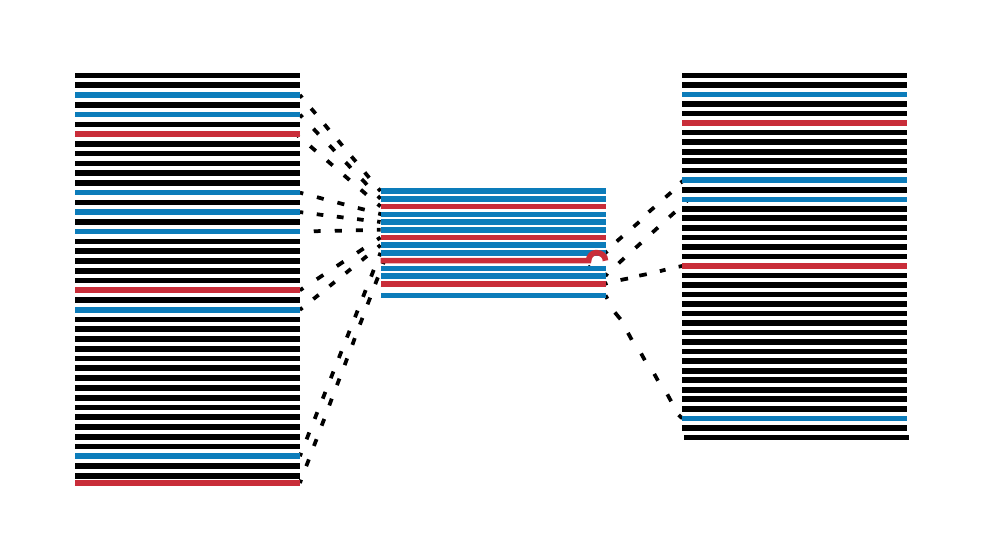
\includegraphics[width=0.4\textwidth]{annotations.png}
\caption{Annotations provide reduced, tractable view of significant events
in a much larger volume of log data.}
\label{f:annotations}
\end{figure}

\begin{itemize}
\item 
\item Temporal and subject (system and component) information are 
      the key fields, along with a human readable description, the 
      annotation itself.
\item The raw logfiles that the annotation concerns should be identified,
      if possible.
\item Multiple people should be able to annotate the same underlying 
      log data, and users of the annotations should be able to 
      identify annotators to request more information, if necessary.  
\item The architectural relationships between components indicated in 
      annotations should be accessible, in order to facilitate 
      traversal from an annotation of interest to annotations relating to
      components that may have impacted it.
\item Annotation fields should support searching based on the subject type 
      of an annotated event (such as a network event) or other 
      related information.
\end{itemize}

%In this subsection we describe the major fields necessary to support the
%architectural requirements that pertain to the annotations themselves
%(as opposed to the remote discovery infrastructure). The prototype
%implementation is an SQLite database, so we descirbe in in terms
%of that implemention, however that is not required. More generally
%this would be descirbed in terms of accessor APIs independent of
%the implementation beneath them.
Our annotation schema is an SQL database definition with a central 
``annotations'' table:

\begin{figure}[H]
\begin{small}
\begin{minted}{sql}
CREATE TABLE 'annotations' (
       id             integer,
       authorid       char(3) NOT NULL,
       description    text NOT NULL,
       -- timespan of the action or event:
       starttime      datetime NOT NULL,
       endtime        datetime NOT NULL,
       -- impact of the action or event:
       startstate     text,
       endstate       text,
       systemdown     boolean,
       system         text,
       components     text,
       -- was the event manually induced?
       manual         boolean,
       -- subject type and annotation context:
       LDcatgroup     text, REFERENCES 'LDgroups'
       LDcategory     text,
       LDtag          text,
       balerpatternid integer,
       -- event source:
       logfiles       text,
       PRIMARY KEY('id','authorid')
        );
\end{minted}
\end{small}
\caption{The central annotations table definition. }
\label{f:ann-table}
\end{figure}

The id, source, description and temporal fields are self-explanatory. 
The impact fields are designed to aid exploratory analysis, for example
\texttt{startstate} and \texttt{endstate} can be used to indicate that
a component that was in a \texttt{faulty} was either \texttt{repaired}
or \texttt{flagged} by the end of the event. A \texttt{systemdown} flag
allows search for events resulting in a full system failure.

The \texttt{system} and \texttt{components} fields correspond to the 
\texttt{Subject} class of the RDF vocabulary.
For the Cray system we define \texttt{node}, \texttt{blade}, \texttt{chassis},
\texttt{cabinet}, \texttt{router}, \texttt{tile}, \texttt{link}, \texttt{nic},
\texttt{smw}, and \texttt{other}, all of which (except \texttt{other}) are 
also \texttt{SubjectType}s described in RDF in data dictionaries and can, in
combination with the \texttt{system}, identify a specific component.

The \texttt{components} may be identified with finer granularity than
is represented in the RDF graph - for example \texttt{c0-1c0s4n0}. One 
envisioned source of machine-generated annotations is LogDiver~\cite{LogDiver}, 
a tool developed by UIUC which associates regular expressions defining
events in log files of interest with categorizations including 
\texttt{node/blade},
\texttt{scheduler}, \texttt{storage}, \texttt{network}, \texttt{cooling/facilities/sensors},
\texttt{power}, \texttt{system software}, \texttt{datawarp}, and \texttt{unknown}.
These also correspond to \texttt{SubjectType}s in an RDF dictionary.

The \texttt{manual} flag indicates that an event was manually induced,
such as an administrator action to take down a node as opposed
to the system taking down a node because it failed a health check.
Knowledge of this can be used to more accurately determine the
number of true failure events and for assessing the effectiveness
and availability of system resilience mechanisms


Note that event may have many relationships. We choose to limit them to one each to address
the requirement of searchability. It is expected that exploration will facilitate dsicovery
of events, even when the first order assocation may be off; also discovery of assocationed
events in different subsytems can help understanding of how events propagate in a system.

Annotations may also refer to other annotations; this is called a \texttt{metaannotation}.
An example might be where an annotation refers to a particular facilities
test and a meta annotations refers to the entire set of tests.

\texttt{Components} can include the compute and any supporting subsystems,
such as storage and facilities related elements. For the Cray system
itself, we define \texttt{node}, \texttt{blade}, \texttt{chassis},
\texttt{cabinet}, \texttt{router}, \texttt{tile}, \texttt{link}, \texttt{nic},
\texttt{smw}, and \texttt{other}.

In order to enable dsicovery of events which are either reported on related
compoentns or that propagate amont components we support the defintion
of \texttt{architectures}. For the Cray system itself, we define three.

The \texttt{physical} architecture consists of parent-child or
container-contained assocations, such as a cabinet is the parent of
3 chassis. For the network components, the router is a child of the blade.
he router is a parent of the links and nics. The physical architecture
can be populated from system defintation (e.g., XE or XC with the
correct number of cabinets for a system).

In order to support the fact that components may be identified by differnet
names in different log messages, an \texttt{alias} table defines those conventions.
This is largely cname, nid, and IP addresses determined from \texttt{/etc/hosts}
or the output for \texttt{rtr --system-map}.

The \texttt{router} architecture includes the network topology information
for the router (e.g., blue:black:green)
for Aries and X:Y:Z for gemini). The router information can be populated from
the system-map output or the otuput of \texttt{rtr --interconnect}.
The \texttt{link} architecture represents the network link connectivity,
consisting of type (e.g., Blue, X+) and the tile endpoints obtained
from the interconnect output.

The \texttt{link} architecuture supports determination if an event affects the
components at teh other end of a network link. The router architecutre
supports determination of proximity of events in the network topology.
We chose to separate architecutres in order to enable different
search and interpreation of events which affect components with
different \texttt{association} with each other. \texttt{associations}
include \texttt{parent-child: component-component} as opposed to
\texttt{parent-child: router tile}, or \texttt{peer: HSN link}
as opposed to \texttt{peer: Router-NIC} or \texttt{peer: NIC-Proc}.
To represent more globally associated, such as SMW
events which can directly affect all components, we define
a \texttt{supremum} relationship.

In the prototype, we define all architectures and relationships,
however we currently prinipally search the physical topology only
and support recursive search up and down, including for supremum
relationships. We are working on tools to better enable search of
the multiple architecture represenations.

In order to determine the effect of events on jobs, we also
intend that job data be made availble with the annotations.
We expect only the current common fields (e.g., starttime,
endtime, components, etc) exposed in scheulder logs or
interfaces.







